\documentclass[11pt,twoside,a4paper]{article}
\usepackage[left=2cm,top=1cm,right=2cm,nohead,nofoot]{geometry}
\usepackage[utf8]{inputenc}
\usepackage{hyperref}
\usepackage{amssymb}
\usepackage{graphicx}
\begin{document}
\author{Jesse Niemistö \and Leo Muona}
\title{Game Engine Architecture: End-term project - Spring 2013 \\
       Technical documentation}

\maketitle

\section{Basic architecture}

The software can be split into two distinct subsystems that have been implemented; animation and physics. Animation subsystem handles skeletal animation (aka forward kinematics), while the physics subsystem is an interface for interacting with 3rd-party physics engine.

Chapters below will take a more in-depth look at the subsystems.

\section{Animation subsystem}

First a lil intro to computer animation. Usually artists animate the characters by only animating the movement of the characters skeletons. This makes animating much easier, as characters might consist tens of thousands of vertices, but only a handful of bones, or joints. Artist only animates the keyframes of the charactes and the computer the fills the 'void', the empty spaces between keyframes, with method called interpolation. After artists have made these animations, they are saved to a file, which then can be read by a software. There might be an huge number of animations, and they all are typically used in different situations. For example when character stands it has different animation than when it is walking. Interpolation between different animations is called crossfade. 

In skeletor a Skeleton class presents a skeleton. Skeleton consists of joints. And these joints form a tree like structure that forms the skeleton. Joint knows it's parent and child joints, so joint knows if it is a leaf or root node. Also this tree like structure makes it easy to recursively traverse skeletons joints. 

SkeletonPose class reflects a single pose of the skeleton in some given time. SkeletonPose class includes a set of transformations for each joint of the skeleton, which are applied to skeletons bind pose to make the pose. This means that only SkeletonPose class is changes when making poses. SkeletonPose class also includes function for crossfading between different animations (poses). The only assumption here is that skeletons that are crossfaded are identical.

COLLADA is an open standard XML schema for exchaning digital assets between various graphics software applications. Skeletor is able to read COLLADA-files with skeletons and animations. Actually only those datas are read as rest are ignored. Collada file structure is outside the scope of this document, but excellent tutorial is available in \url{http://www.wazim.com/Collada_Tutorial_1.htm}

\begin{figure}
  \centering
    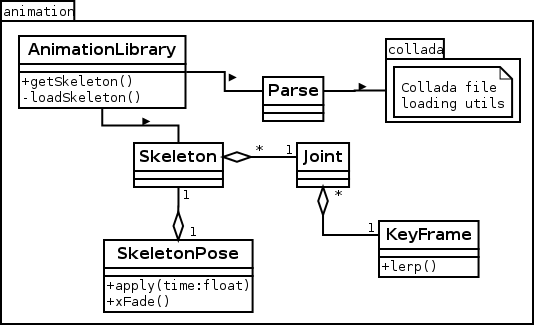
\includegraphics[scale=0.7]{animation_subsystem.png}
  \caption{animation subsystem architecture}
  \label{animsubsys}
\end{figure}

The figure~\ref{animsubsys} shows the basic architecture of the animation subsystem. The figure represents the classes defined under src/animation/ directory. AnimationLibrary class is used to load skeleton from external files. It will call the load function from Parse class, which will call proper loader depending on file extension, though only COLLADA is supported.

\section{Physics subsystem}

Animation has it's uses and character death can be done with dramatic death animations. But after that, a game engine should handle dead bodies, as well as other objects, with certain realism. This is "easy" to obtain with implementing some physics API to the project, and in this case it is Bullet Physics. Bullet Physics engine is an open source 3D physics engine, that has support for collision detection, soft body dynamics and rigid body dynamics. It has been developed mainly by Erwin Coumans and is published under zlib licence.

In skeletor we use Bullet Physics engine to calculate skeleton's physics "after death". This is done by converting player's SkeletonPose into BulletRagdoll. Then the ragdoll is inserted into btDynamicsWorld and for each time the main loop is ran, physics world is also updated. In an optimal situation the ragdoll is converted back to Skeletor's SkeletonPose form before rendering frame.

Physics subsystem also supports boxes for couple reasons. Firsly, you can easily build a floor for the world with boxes. Secondly, physics engine is easy to get started with a few boxes, thus making sure the time simulation and basic settings are working correctly. Same rules apply for boxes that apply for skeletons. That is, boxes have to be converted from Bullet form to Skeletor form inside the main loop for correct rendering.

\begin{figure}
  \centering
    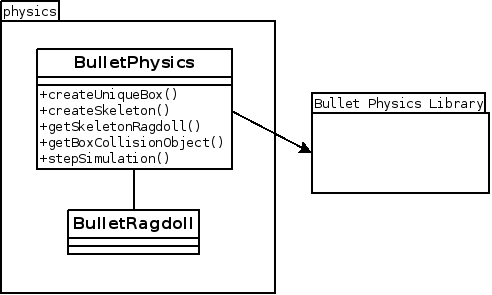
\includegraphics[scale=0.7]{physics_subsystem.png}
  \caption{physics subsystem architecture}
  \label{physicssubsys}
\end{figure}

The figure~\ref{physicssubsys} shows how the Bullet Physics library is used with Skeletor's physics classes. The figure has only main functions (initialization \& debug functions are missing), thus the it's main function is to just visualize the previous texts. The bullet integration is developed in a way that it could "easily" be replace by other physics engine in the software.

At current state the physics implementation is not working correctly with skeletons, thus it should serve as a basis for future development.

\section{Known bugs and limitations}

Here is the list of known bugs and limitations on the software.

\begin{itemize}
  \item Collada
  \begin{itemize}
    \item Collada files must have at least and at most one skeleton.
    \item Root joint of the skeleton must be named as 'root'.
    \item Only Maya and blender exported collada files work and has been tested.
    \item Only library\_animation and library\_visual\_scene nodes are read, meaning character meshes are not read nor rendered.
    \item Only supported (and tested) version of collada schema is 1.4.1. Other versions are untested.
  \end{itemize}
  \item Animation crossfading only works with identical skeletons.
  \item KeyFrame animation assumes that interpolation is linear, no bezier is supported.
  \item Turning camera too far up or down distorts the scene, proper way of handling would be to put degrees of freedom to camera movement.
  \item Physics system and animation system has no real interaction, there is no inverse kinematics!
  \item Physics
  \begin{itemize}
    \item Converting skeleton to ragdoll does not create bones/joints in correct locations.
    \item Because of previous, converting from ragdoll to skeleton has not been implemented.
    \item Ragdolls does not have gravity for time being. After conversion errors are fixed, gravity can be turned on.
    \item Boxes can be created into gravity system only in upwards-position. (not tilted)
    \item Joint conversion has to uses Skeletor's default joint angle values given in animation::Joint constructor.
  \end{itemize}
\end{itemize}

\end{document}
